\documentclass{exam}

%%%%%%%%%%%%%%%%%% PACKAGES %%%%%%%%%%%%%%%%%%%%%%%%

\usepackage{amsmath}
\usepackage{amsfonts}
\usepackage{tcolorbox}
\usepackage{tikz,tkz-euclide,tikz-3dplot}

%%%%%%%%%%%%%%%%%% HEADER AND FOOTER %%%%%%%%%%%%%%%

\pagestyle{headandfoot}
\firstpageheadrule
\runningheadrule
\firstpageheader{\S3.F.3 - Rates of Change}{}{AP Precalc\\Mr. Carey}
\runningheader{\S3.F.3}{}{Mr. Carey}
\firstpagefooter{}{}{}
\runningfooter{ }{\thepage}{ }

%%%%%%%%%%%%%%%%%%%%%%%%%%%%%%%%%%%%%%%%%%%%%%%%%%%%

\begin{document}
\section*{Rates of Change of Polar Functions}
Due to the nature of changing variables, talking about rates of change requires slightly more focus. This is becuase our normal understanding of the rate of change can be interpreted as\dots
\[\text{Rate of Change}=\frac{\Delta y}{\Delta x}=\frac{\text{rise}}{\text{run}}.\]
However, when it comes to polar coordinates, it could be different.

\begin{tcolorbox}[title=Defintion: \textit{Rates of Change in Polar Coordinates},title filled,colframe=black,sharpish corners,width=\linewidth]
    Let $r=f(\theta)$ be a polar function. Then, the \textbf{rate of change of} $r$ can be interpreted as 
    
    \begin{minipage}[t]{.45\linewidth}
        \[\displaystyle\frac{\Delta r}{\Delta \theta}\]

        This is the rate of change of $r$ with respect to $\theta$. We determine this by considering ''as $\theta$ increases, does $r$ increase or decrease?''
    \end{minipage}
    \hfil
    \begin{minipage}[t]{.45\linewidth}

        \[\displaystyle\frac{\Delta y}{\Delta x}\]

        This is the rate of change of $y$ with respect to $x$. As $\theta$ and $r$ change, is the point going up or down in relation to the $x$-axis?
        
    \end{minipage}


    \begin{center}
        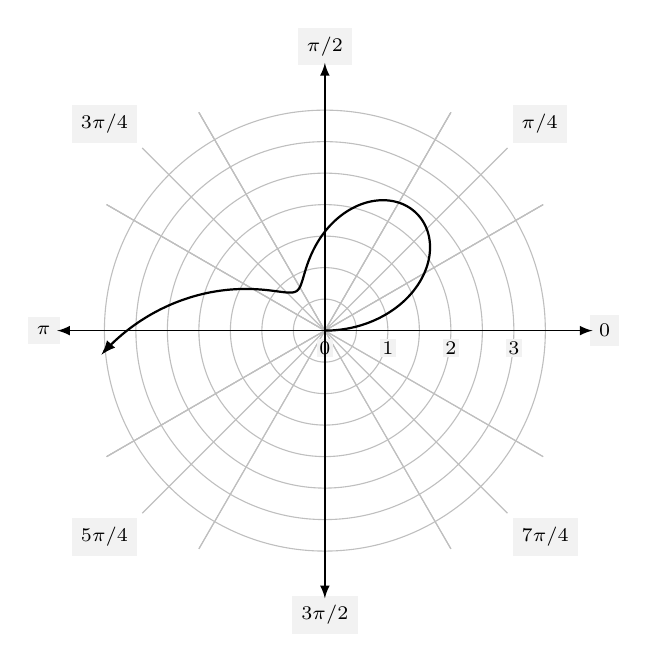
\begin{tikzpicture}[scale=.8]
             

            % Draw the lines at multiples of pi/6
            \foreach \ang in {0,...,31} {
                \draw [lightgray] (0,0) -- (\ang * 180 / 6:4);
            }
            
            % Add the labels at multiples of pi/4
            \foreach \ang/\lab/\dir in {
            0/0/right,
            1/{\pi/4}/{above right},
            2/{\pi/2}/above,
            3/{3\pi/4}/{above left},
            4/{\pi}/left,
            5/{5\pi/4}/{below left},
            7/{7\pi/4}/{below right},
            6/{3\pi/2}/below} {
            \draw [lightgray] (0,0) -- (\ang * 180 / 4:4.1);
            \node [fill=black!5!white] at (\ang * 180 / 4:4.2) [\dir] {\scriptsize $\lab$};
            }
            
            % Concentric circles and radius labels
            \foreach \s in {0, 1, 2, 3} {
            \draw [lightgray] (0,0) circle (\s + 0.5);
            \draw [lightgray] (0,0) circle (\s);
            \node [fill=black!5!white] at (\s, 0) [below=1mm,inner sep=1pt] {\scriptsize $\s$};
            }

            \draw[latex-latex,semithick](-4.25,0)--(4.25,0);
            \draw[latex-latex,semithick](0,-4.25)--(0,4.25); 

            \draw[domain=0:3.25,samples=200,smooth,-latex,thick,] plot ({deg(\x)}:{\x+1.5*sin(2*(\x r))});

        \end{tikzpicture}
    \end{center}

\end{tcolorbox}

\noindent Consider the polar function $r(\theta)=3\cos3\theta$. Graph this function on your calculator and locate the points at the specified values of $\theta$. Is the value of $r$ increasing or decreasing over this interval?
\begin{parts}
    \part $\displaystyle\theta=\frac{\pi}{6}$,

    \vspace{\stretch{1}}

    \part $\displaystyle\theta=\frac{\pi}{4}$,

    \vspace{\stretch{1}}

    \part $\displaystyle\theta=\frac{\pi}{3}$.

    \vspace{\stretch{1}}

\end{parts}


\newpage
\begin{tcolorbox}[title=Defintion: \textit{Distance from the Origin},title filled,colframe=black,sharpish corners,width=\linewidth]
    Let $r=f(\theta)$ be a polar function. Then the distance from the origin is \textbf{increasing} when either
    \begin{itemize}
        \item $r$ is positive and increasing
        \item $r$ is negative and decreasing
    \end{itemize}
    Similarly, the distance from the origin is \textbf{decreasing} when either
    \begin{itemize}
        \item $r$ is positive and decreasing
        \item $r$ is negative and increasing
    \end{itemize}

\end{tcolorbox}
\subsection*{Examples}

\begin{questions}
    \question Consider the curve gievn by $\displaystyle r=3$ on the interval $0\le \theta\le2\pi$.
        
        \begin{parts}
            \part Sketch a graph of the curve $r$.

            \part What is the rate of change of $r$ with respect to $\theta$? How do you know?

            \vspace{\stretch{1}}

            \part For what interval(s) of $\theta$ is $y$ increasing?

            \vspace{\stretch{1}}

        \end{parts}

    \begin{minipage}[b]{.45\linewidth}
        \question The graph of $r(\theta)=1-2\cos\theta$ is shown alongside. Determine if the polar curve is getting closer to the origin, futher from the origin, or neither when $\theta=\pi/6$.
    \end{minipage}
    \hfill
    \begin{minipage}{.45\linewidth}

        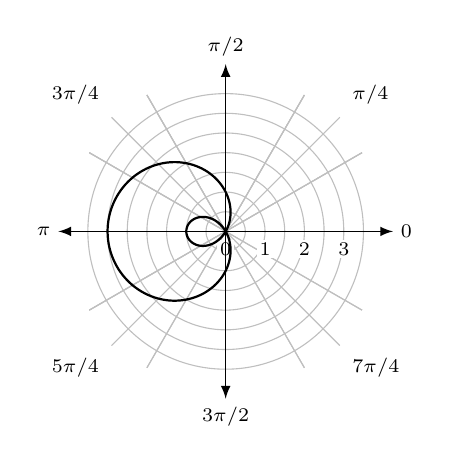
\begin{tikzpicture}[scale=.5]
            % Draw the lines at multiples of pi/6
            \foreach \ang in {0,...,31} {
                \draw [lightgray] (0,0) -- (\ang * 180 / 6:4);
            }
            
            % Add the labels at multiples of pi/4
            \foreach \ang/\lab/\dir in {
            0/0/right,
            1/{\pi/4}/{above right},
            2/{\pi/2}/above,
            3/{3\pi/4}/{above left},
            4/{\pi}/left,
            5/{5\pi/4}/{below left},
            7/{7\pi/4}/{below right},
            6/{3\pi/2}/below} {
            \draw [lightgray] (0,0) -- (\ang * 180 / 4:4.1);
            \node [fill=white] at (\ang * 180 / 4:4.2) [\dir] {\scriptsize $\lab$};
            }
            
            % Concentric circles and radius labels
            \foreach \s in {0, 1, 2, 3} {
            \draw [lightgray] (0,0) circle (\s + 0.5);
            \draw [lightgray] (0,0) circle (\s);
            \node [fill=white] at (\s, 0) [below=1mm,inner sep=1pt] {\scriptsize $\s$};
            }

            \draw[latex-latex,semithick](-4.25,0)--(4.25,0);
            \draw[latex-latex,semithick](0,-4.25)--(0,4.25); 

            \draw[domain=0:6.4,samples=200,smooth,thick,] plot ({deg(\x)}:{1-2*cos((\x r))});
        \end{tikzpicture}
        
    \end{minipage}
    
        



    \vspace{\stretch{1}}

    For the example above, is there another way we can visualize the rate of change of $r$ with respect to $\theta$?

    \vspace{\stretch{.5}}

    \newpage

    \begin{tcolorbox}[title=Defintion: \textit{Average Rate of Change of a Polar Function},title filled,colframe=black,sharpish corners,width=\linewidth]
        Let $r=f(\theta)$ be a polar function. Then the average rate of change of $r$ on the interval $[\theta_1,\theta_2]$ is given by
        \[\Delta r=\frac{f(\theta_2)-f(\theta_1)}{\theta_2-\theta_1}.\]
    \end{tcolorbox}

    \question Consider the curve given by $r=-3+5\sin\theta$ on the interval $0\le \theta\le 2\pi$.

    \begin{parts}
        \part Is the distance between $f(\theta)$ and the origin increasing or decreasing on the interval $\pi/2\le\theta\le3\pi/4$? 

        \vspace{\stretch{1}}

        \part Find the average rate of change of $f(\theta)$ between $\theta=\pi/4$ and $\theta=\pi/2$.

        \vspace{\stretch{1}}

    \end{parts}

    \begin{minipage}{.65\linewidth}
        The table alongside gives select values of a polar curve $r$.
        \begin{parts}
            \part Is $r$ increasing or decreasing on the interval $\displaystyle\frac{\pi}{4}\le\theta\le\frac{\pi}{2}$?

            \vspace{\stretch{.5}}

            \part Is the distance betwen $f(\theta)$ and the pole increasing or decreasing on the interval $0\le\theta\le\pi/4$?

            \vspace{\stretch{.5}}

            \part Is the rate of change of $r$ faster on the interval $\left[0,\frac{\pi}{8}\right]$ or $\left[\frac{\pi}{8},\frac{\pi}{4}\right]$? Justify your answer.

            \vspace{\stretch{.5}}

        \end{parts}
    \end{minipage}
    \hfill
    \begin{minipage}{.25\linewidth}
        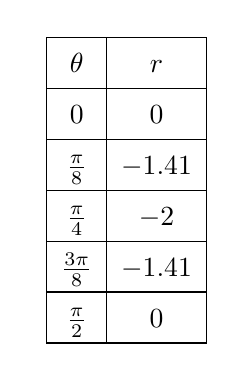
\begin{tikzpicture}[scale=1.5]
            \node at (0,0) {
              \renewcommand{\arraystretch}{1.5} % Adjusts the row height
              $\begin{array}{|c|c|}
                \hline
                \theta & r \\
                \hline
                0 & 0\\
                \hline
                \frac{\pi}{8} & -1.41 \\
                \hline
                \frac{\pi}{4} & -2\\
                \hline
                \frac{3\pi}{8} & -1.41\\
                \hline
                \frac{\pi}{2} & 0\\
                \hline
              \end{array}$
            };
          
            % Additional TikZ commands for customizing the table, if needed
          \end{tikzpicture}
    \end{minipage}

    \vspace{\stretch{1}}

\end{questions}






\end{document}